\begin{figure}[htp]
 \centering
 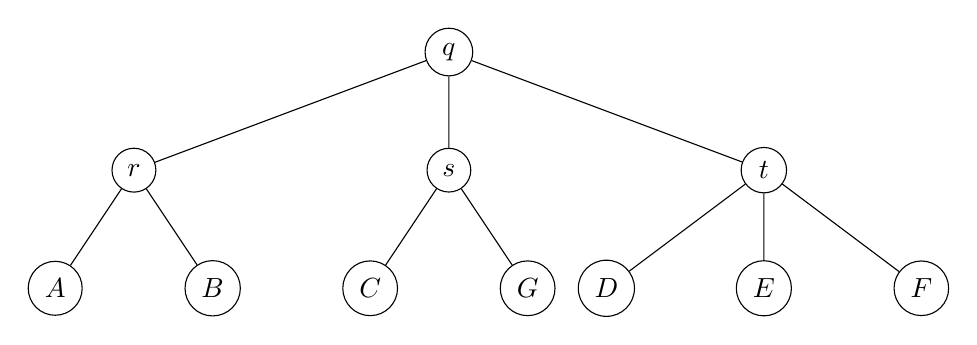
\begin{tikzpicture}[level/.style={sibling distance = 40mm/#1}]
  \node[circle,draw] (z){$q$}
    child {node [circle,draw] (a) {$r$}
     child {node [circle,draw] (b) {$A$}}
     child {node [circle,draw] (c) {$B$}}
    }
    child {node [circle,draw] (d) {$s$}
     child {node [circle,draw] (e) {$C$}}
     child {node [circle,draw] (f) {$G$}}
    }
    child {node [circle,draw] (g) {$t$}
     child {node [circle,draw] (h) {$D$}}
     child {node [circle,draw] (i) {$E$}}
     child {node [circle,draw] (j) {$F$}}
    };
 \end{tikzpicture}
 \caption{Objektijoukosta muodostettu BVH-puu}
 \vspace{-0.5cm}
 \label{bvhtree}
\end{figure}
